\documentclass[runningheads]{llncs}
\usepackage{graphicx}
\usepackage{algorithmic}
\usepackage[ruled,vlined]{algorithm2e}
\usepackage{booktabs,chemformula}
\usepackage{cite}
\usepackage{graphicx,tabularx}
\usepackage{array}
\usepackage{balance}
\usepackage{geometry}
\geometry{
a4paper,
 total={170mm,257mm},
 left=40mm, right=40mm,
 top=20mm,
 }
\PassOptionsToPackage{hyphens}{url}
\usepackage{url}


\def\BibTeX{{\rm B\kern-.05em{\sc i\kern-.025em b}\kern-.08em
    T\kern-.1667em\lower.7ex\hbox{E}\kern-.125emX}}

\begin{document}

\title{A Case Study to Evaluate the Usability, Based on Cognitive Method:E-Bus ticket}

\author{Raihan Ahmed\inst{1}\orcidID{19202103480/44} \and
Humyra Ayesha \inst{2}\orcidID{19201103470/44} \and
Umma Shanjida Tasmim\inst{3}\orcidID{19201103442/44} \and
Md. Saidur Rahman Hasib\inst{4}\orcidID{19202103043/44}}
% %
\authorrunning{Md. Raihan Ahmed}

\institute{Bangladesh University of Business and Technology, \\Dhaka-1216, Bangladesh. \\} 

\maketitle              
\begin{abstract}
E-Bus ticket, a web based application which works with the ticket management system  used in the bus ticket purchasing process. It Presents a review on Online Ticketing Platform used in bus transport management, facility for seat reserving or canceling reservations and Instant communication with transport companies or agencies. Traditional database, ticket booking and OBTRS was developed to computerize buses and it maintains customer details, bus and reservation details etc. The total report contains the software Structured Systems Analysis, Design Methodology and use of user experiences. This Software is used with PHP hypertext protocol language which is used for the front-end of the software and the back-end was designed with MySQL. As a result, the software is capable of improving the customer's choice and  managing customers' daily needs of arriving in buses. Despite the current functionality of the software, adding the functionality such as customer Use of email to send tickets, Ticket verification, bus location etc. should be implemented in this system. Hence, other activities should be integrated to improve the bus e-ticketing system.

\keywords{Cognitive method  \and  \and e-ticket \and Risk management \and Usability.}
\end{abstract}

\section{Introduction}
E-ticketing is the most used platform in the current era of the world. People in different areas like villages, urban and metro sites are now using this global platform for making their life better and easier. From students to professionals everyone is using buses for transportation to reach their destinations on time. As there are multiple routes across the city, it can take just the right amount of time to arrive at their destination. Due to the demand of bus transport among the public, many facilities are being provided for the comfortable travel of all types of passengers. Although the luxury sector has improved, the ticketing systems to purchase the tickets of buses by  e-ticketing platform. There will usually occur fights, arguments and problems between bus conductors and passengers for misunderstandings of the right amount of money for arriving. Therefore, an online system will be introduced to facilitate currency exchange and transactions in public bus transport to solve this kind of problem. and make the processes easier.
\\\\
At present, the best example in our city, Dhaka, is going to introduce an e-ticketing system after 16th December, the opening of Metro-Rail. In this sector electronic ticketing machines are used to collect tickets to arrive at their destination by metro. And, similarly we are using this kind of software to book tickets anywhere in the city by their smartphone and also from ticket counters.\\
The key contributions of our software in the report are following: 
\begin{itemize}
    \item We are developing our software by taking user experiences by users and trying to solve the problems and made e user friendly software to use.
    \item Making a user friendly software take their feedback's, remark positive-negative comments and going to solve those problems.
    \item Our software can be beneficial for the passengers who uses bus for transpiration's in their daily life and also for the bus agencies.
\end{itemize}

The rest of the part of this paper is organized in the following manner. Section \textbf{2} describes the project Literature review of our proposed work. Section \textbf{3} provides project Methodology. We show some experimental result analysis in section \textbf{4}.
\section{Literature Review}
Katarzyna Stawarz et al are works on Cognitive Behavioral Therapy Apps for Depression. Though many applications make the claim to be based on CBT for depression, few of these claims have any supporting evidence. App creators should be able to explain the therapeutic benefits of their works. To offer a positive user experience, they should also employ strategies that are supported by evidence. There was also no link between the presence of expert involvement and user ratings.
Mahdi Ebnali et al are work on an application in Highly Automated Driving Training Driving performance was considerably improved by VR and serious gaming training programs, which led to shorter time-to-collision (TTC), longer time-to-collision (TOT), and fewer collisions. Comparatively to the control group, participants in training groups reported more calibrated trust and less unpredictable acceptance. Depending on the extent of automation, autonomous vehicles may increase road safety by helping drivers in a variety of ways. The strength of generalizability is diminished by a limited sample size and imbalanced gender ratio. In a follow-up study, we'll take into account another training group with a concentration on traditional training.
Amir Dirin et al work on in mobile augmented reality Mobile augmented reality (MAR) as a significant interactive technology is gaining significant traction. User Experience elements that support the acceptance of mobile augmented reality applications have received little attention. The purpose of this study was to understand how users emotionally interpret MAR apps and to pinpoint potential and problems related to MAR applications.
Shabnam Kazemi et al are created a Survey on the Usability and User Experience of the Open Community Web Portals.
Information sharing platforms and public community web portals are the subject of a study on usability and user experience research. The study's objective was to give a summary of how usability has been discussed in the literature in relation to information-sharing web portals. Our research was utilized by the SPEED (Smart Ports Entrepreneurial Ecosystem Development) project. 27 out of the 42 articles that were chosen used some type of usability-testing or web portal evaluation. This might seem like a small amount, however usability may not have been the main topic of the research in the remaining papers.

Mulholland et al worked on Semiotic Interface sign Design and Evaluation (SIDE) framework.\\
\vspace{4.5 in}
\section{Project Methodology}
A methodology is a set of ideas or guidelines about how to proceed in gathering and validating knowledge of a subject matter. Different areas of science have developed very different bodies of methodology on the basis of which to conduct their research. Here, We have focused on designing a software which will outcomes the problems of purchasing tickets, avoid inconvenience situation and a user friendly software.


\begin{figure}[h]
\centerline{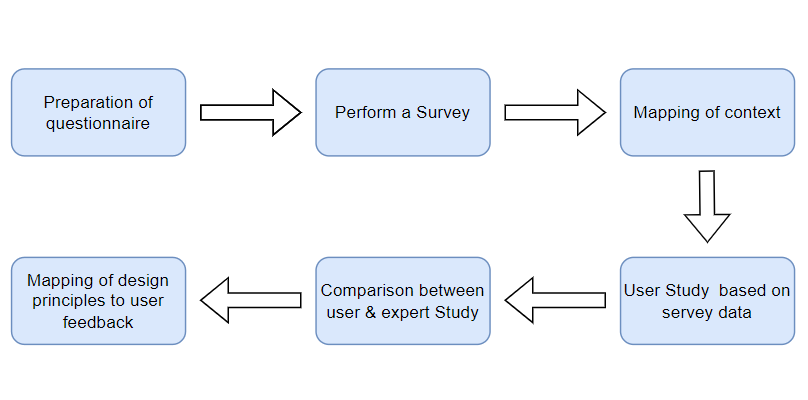
\includegraphics[width=\textwidth]{context diagram of eticket.png}}
\caption{Methodological approach in e-bus ticketing}
\label{fig}
\end{figure}

\subsubsection{Prepare of questionnaire}
This is a fact finding technique used for gathering broad information from large group of
potential users, it’s often consist of set of written questions. Questionnaire is to select
individuals whom the questionnaire will be distributed to. Those individuals should be selected
from those who are using the system or related to the system. In this report students are the
users of the system and therefore the questionnaire will be given to 33 students of BUBT.

\subsubsection{Perform a survey}
We selected 33 participants in our survey(12 females and 19 male) their average age scale is about 20-25 years old. They were all enrolled undergraduate program in Bangladesh University of business and Technology. We take survey with online survey platform named Google Form.

\subsubsection{Context Mapping}
We conducted the survey and then the context mapping. We linked context 1 to action domains . In C2,C4,C5,C7 we works for engagement also we linked C3,C5,C6,C7 to goal domain. We have prepared a total of 12 questions of control, engagement, goal domain, so we mapped it to those three domains.
\subsubsection{User study based on survey data}
As we conduct a survey with 33 people. Everyone gave their review. Here we found a average of survey question based on User data.
\subsubsection{Mapping of design principles to user feedback}
Compare users Comments and question ratings and find the best and worst things in the software to make the solutions.
\newpage
\subsection{Questionnaire and context mapping}
We have prepared a total of 12 questions where 4 questions is for action domain, 5 for control and 3 for goal domain.\\And also added a additional question where a user can give their comments about the website good or bad. They can give suggestions through this.
\begin{figure}[h]
\centerline{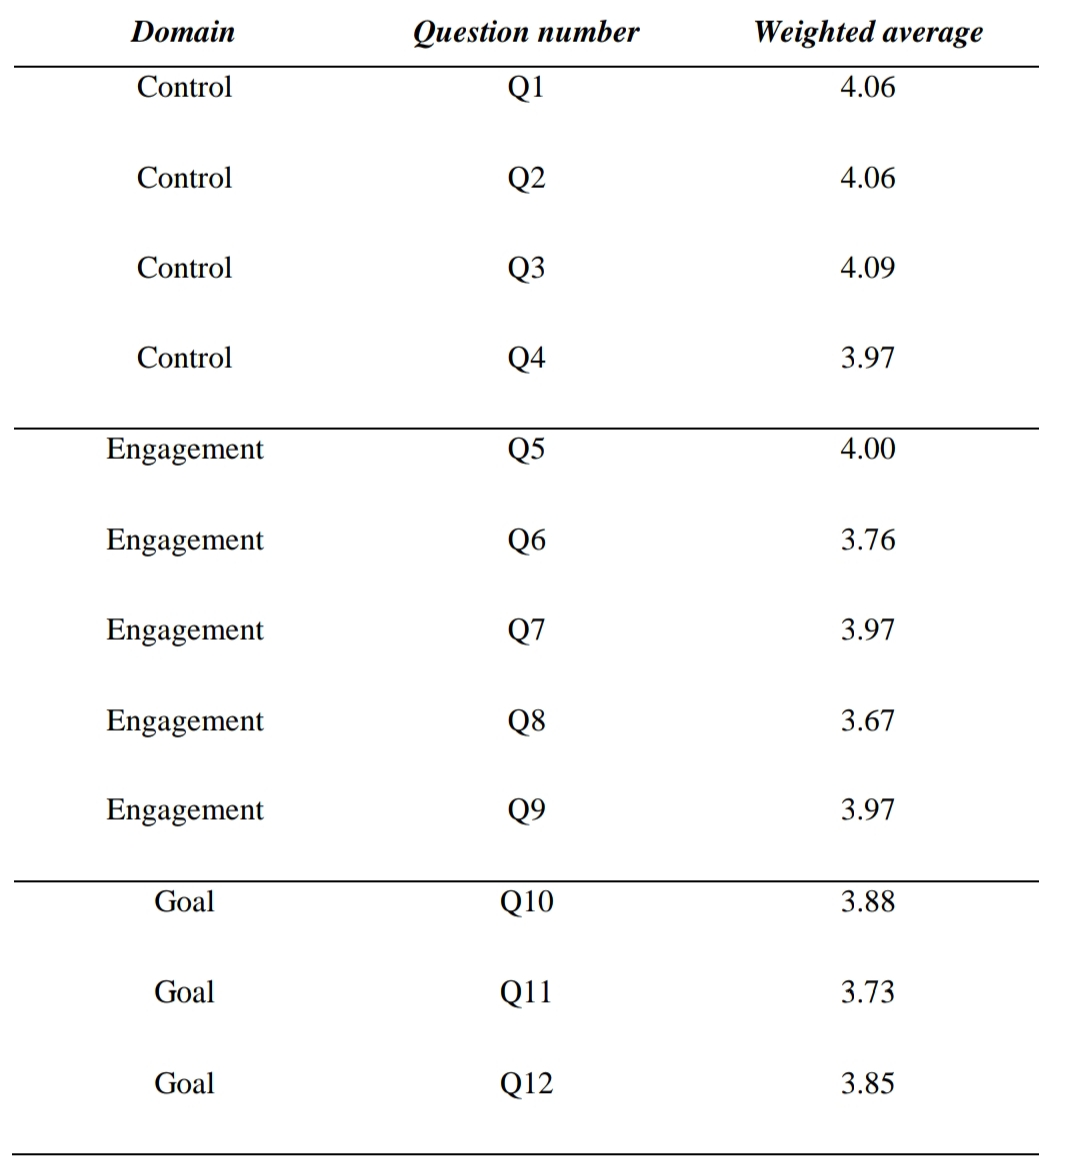
\includegraphics[width=3 in]{question average.jpg}}
\caption{The weighted average score of survey feed-backs}
\label{table}
\end{figure}

And we added a Radar chart of the average scores of different questionnaires in the survey.
\begin{figure}[h]
\centerline{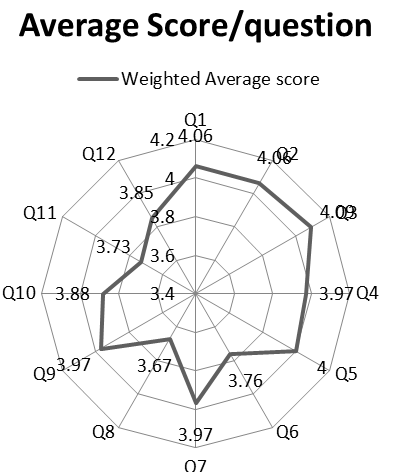
\includegraphics[width=2.5 in]{average score.png}}
\caption{Radar Diagram of average scores}
\label{fig}
\end{figure}
\vspace{1in}
\\Here added a line chart of per question-wise score of questionnaire's-
\begin{figure}
    \centering
    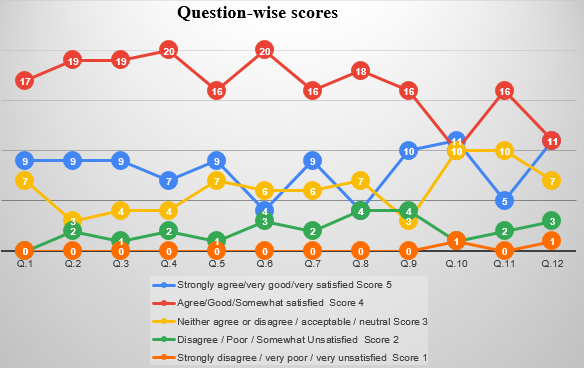
\includegraphics[width=5 in]{img/rename.png}
    \caption{Question wise scores}
    \label{fig:my_label}
\end{figure}
%\vspace{1in}
\subsubsection{Context mapping}
is a tool that allows you to identify the relationship between bounded contexts and the relationship between the teams that are responsible for them.\\Here, added a context map and context mapping diagram(total-score and average score) in fig 4 and fig 6:
\begin{figure}[h]
\centerline{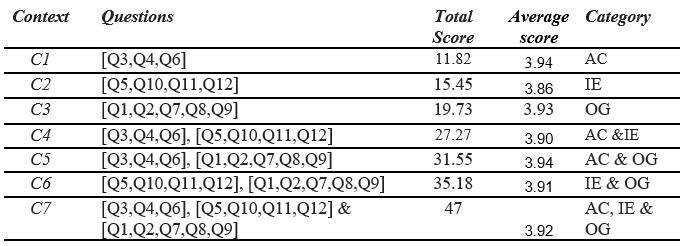
\includegraphics[width=5 in]{Context chart.png}}
\caption{Context mapping}
\label{fig}


\end{figure}
\begin{figure}[h]
    \centering
    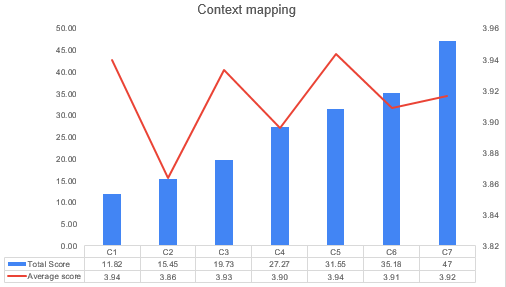
\includegraphics[width=5 in]{Context mapping.png}
    \caption{Context Mapping chart}
    \label{fig:my_label}
\end{figure}

\vspace{3in}
\subsection{Highlighted user feedback}
where P Denotes the positive feedback and n denotes negative feedback.
\begin{figure}[h]
\centerline{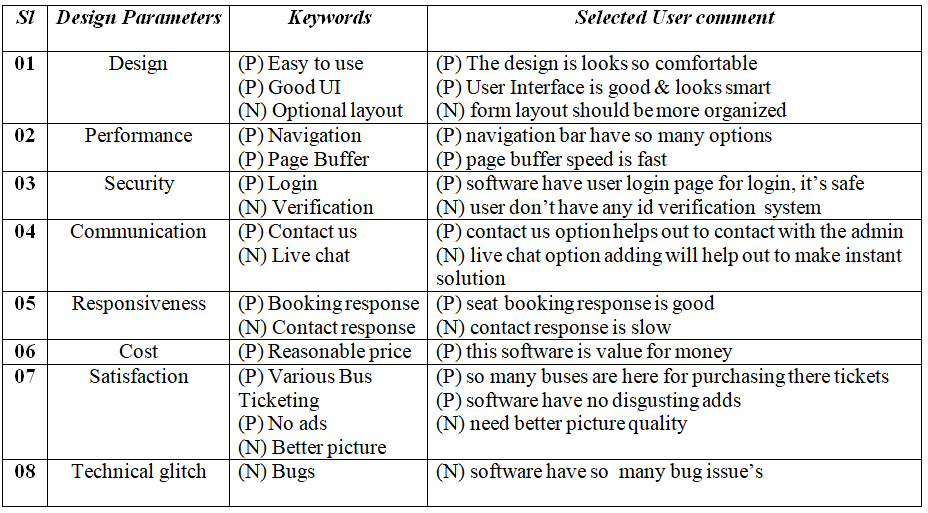
\includegraphics[width=5 in]{highlightes.png}}
\caption{The Highlighted positive And negative feed-backs from the users in survey}
\label{fig}
\end{figure}
\subsubsection{Communication}: We both found positive and negative comments on communication parameters. We get positive feedback for our best customer care support and negative feedback for not having Live chat feature.
\subsubsection{Satisfaction:} In satisfaction parameters we define users' satisfaction level. They were very much satisfied to this website.
\subsubsection{Responsiveness:} Users satisfaction on responsiveness parameter for seat booking. But contact responsive is slow.

\subsubsection{Performance:}so many options provided so-that we got positive feedback in the parameters of performance. Also page buffer speed is good. There was no negative feedback. \subsubsection{Technical glitch:} In this parameter we get negative feedback for some bug issues. But here we get negative feedback more than positive.. Negative feedback was provided because of software bugs.
\subsubsection{Cost:} Positive feedback was provided in this area because of the reasonable pricing.
\newpage
\section{Implementation}
As a result of this research, the model for e-ticketing buses, the implementation
of some activities, the existence of activities, actions or processes of a system, a
planned activity, and structure. To explain the proposed system, diagrams are
used. A use case diagram is a diagram that represents interactions between use
cases and actors.
\begin{align}
    \textbf{Web site Page Screenshot}
\end{align}



\begin{figure}[h]
    \centering
    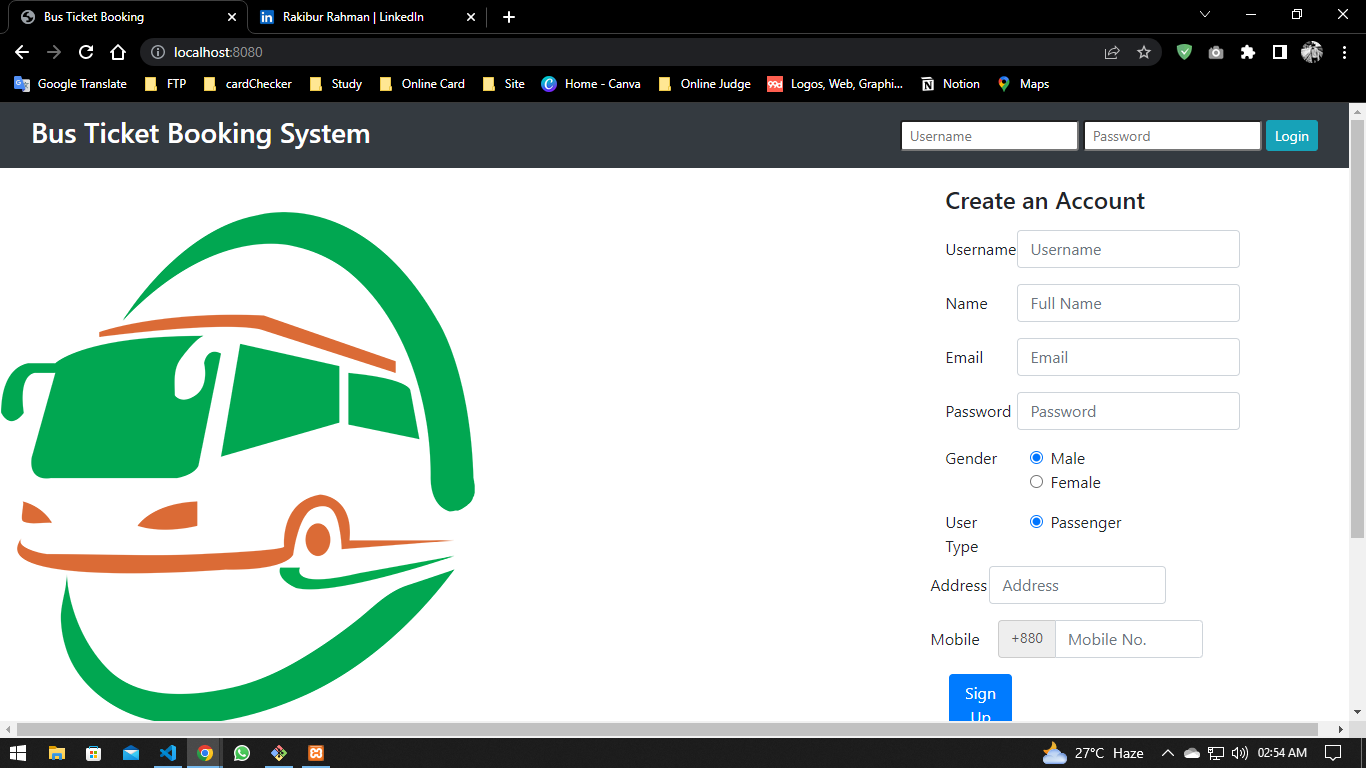
\includegraphics[width=10cm,height=8cm]{img/homepage.png}
    \caption{Home Page}
    \label{fig:my_label}
\end{figure}
\begin{figure}[h]
    \centering
    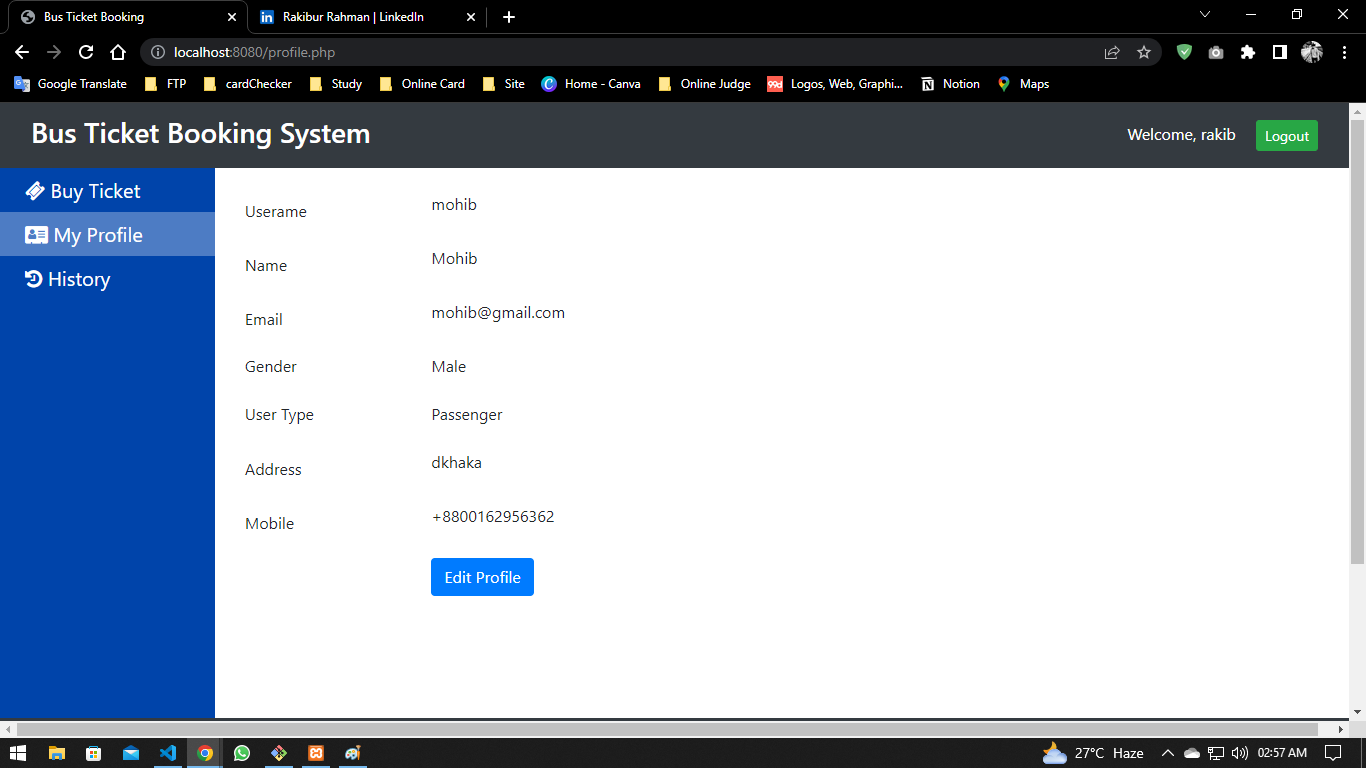
\includegraphics[width=10cm,height=8cm]{img/customer profile.png}
    \caption{Customer Profile}
    \label{fig:my_label}
\end{figure}
\begin{figure}[h]
    \centering
    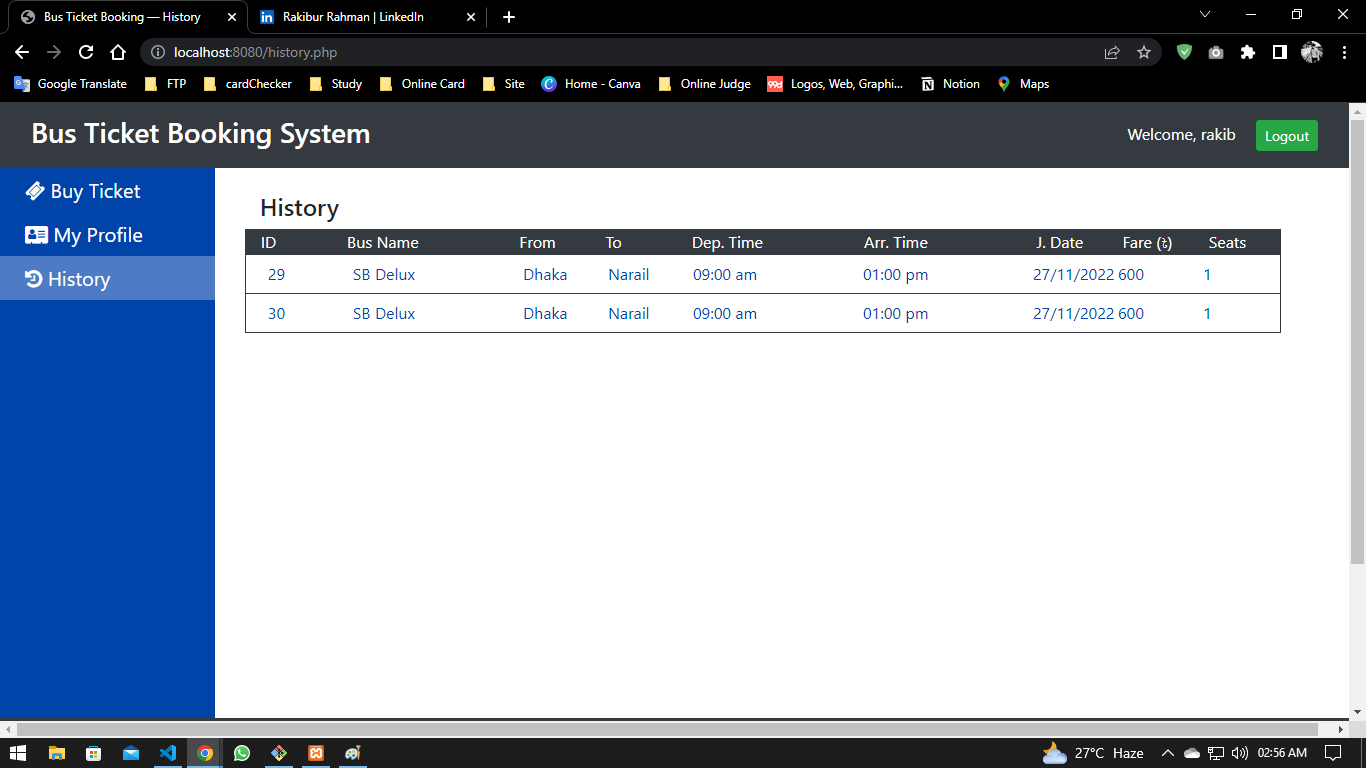
\includegraphics[width=10cm,height=8cm]{img/customer history.png}
    \caption{Customer History}
    \label{fig:my_label}
\end{figure}
\begin{figure}[h]
    \centering
    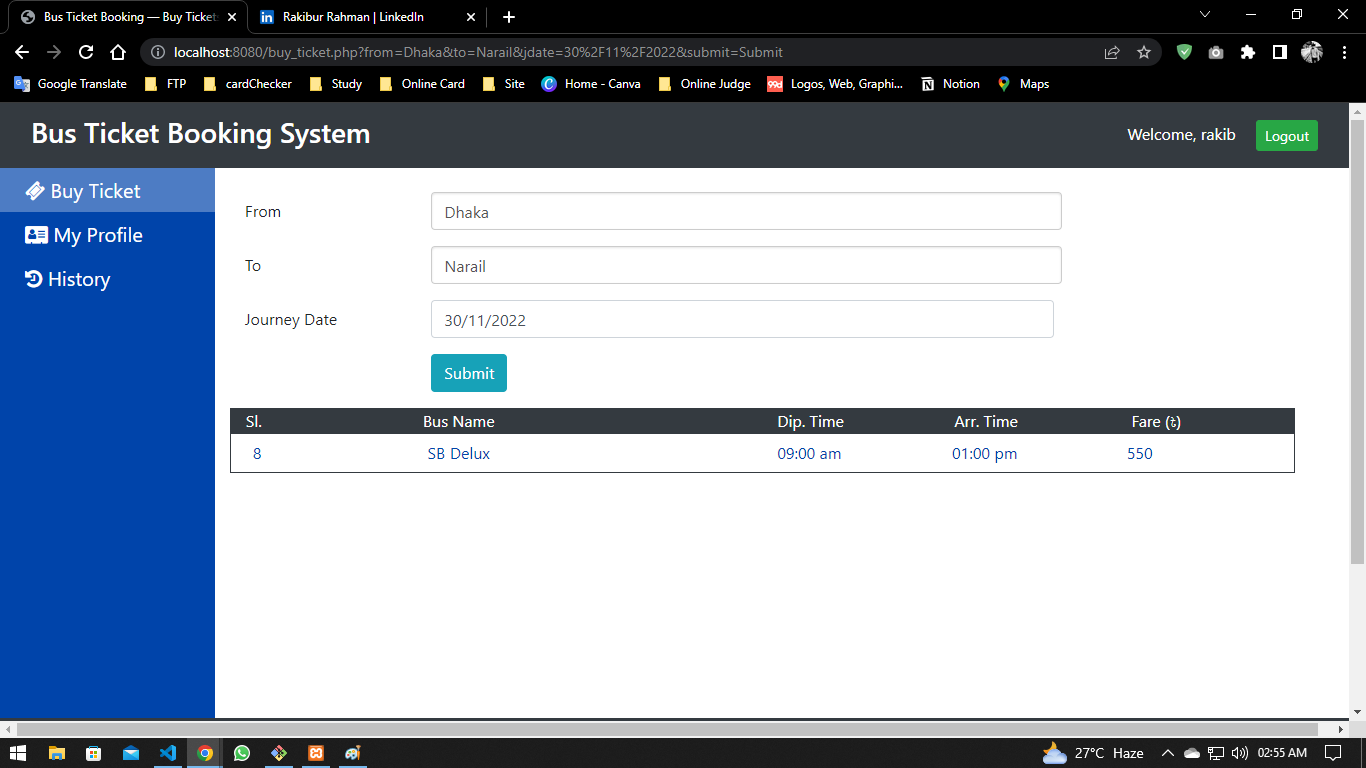
\includegraphics[width=10cm,height=8cm]{img/bussearch.png}
    \caption{Bus Search}
    \label{fig:my_label}
\end{figure}
\begin{figure}[h]
    \centering
    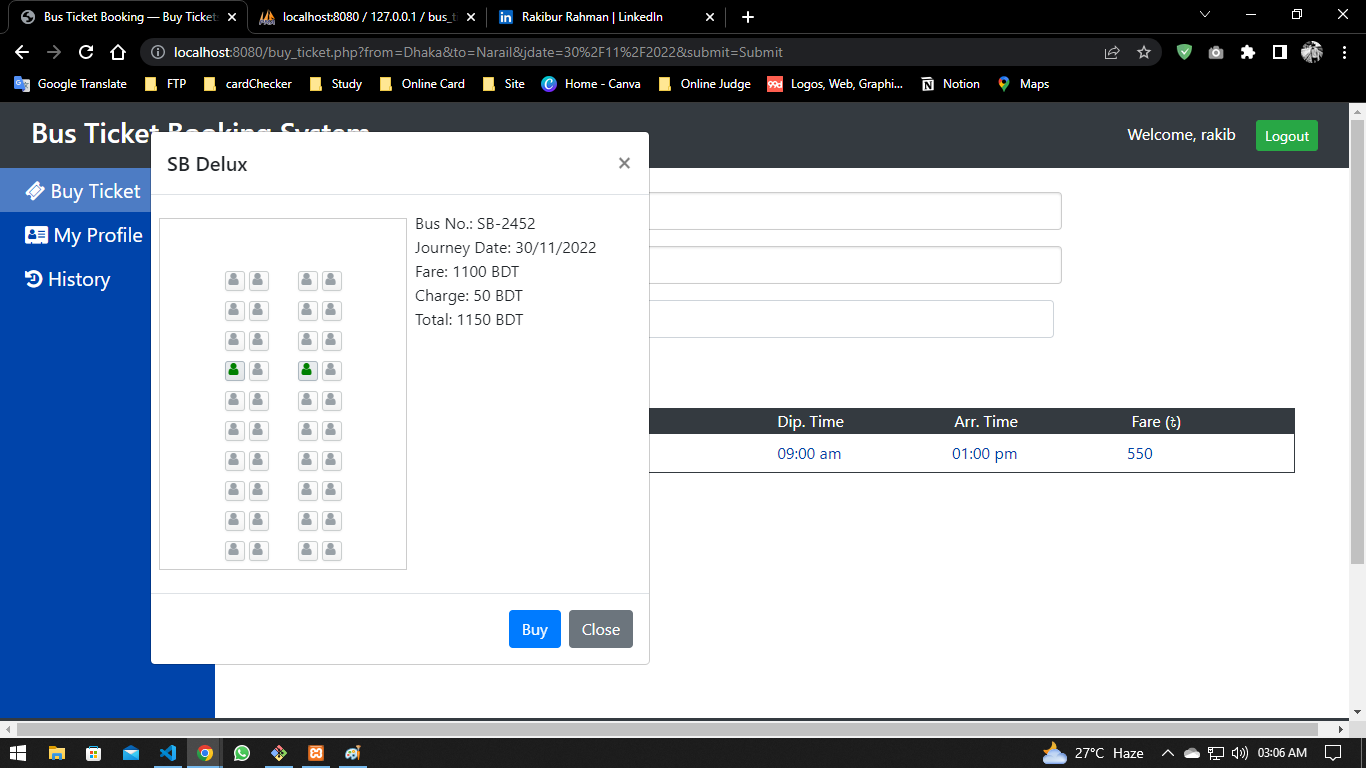
\includegraphics[width=10cm,height=8cm]{img/purchase ticket.png}
    \caption{Choose seat}
    \label{fig:my_label}
\end{figure}
\newpage
\begin{figure}[h]
    \centering
    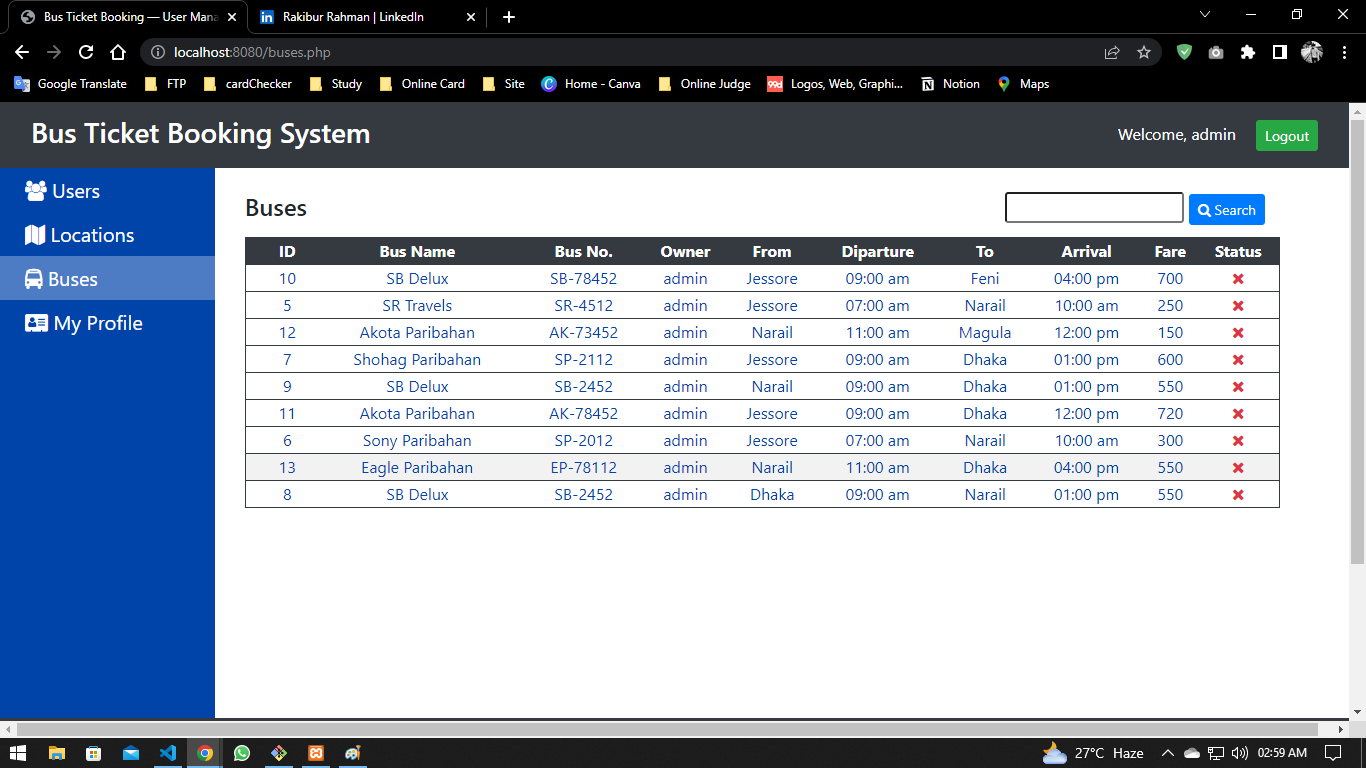
\includegraphics[width=10cm,height=8cm]{img/admin view bus.png}
    \caption{Admin View bus}
    \label{fig:my_label}
\end{figure}
\begin{figure}[h]
    \centering
  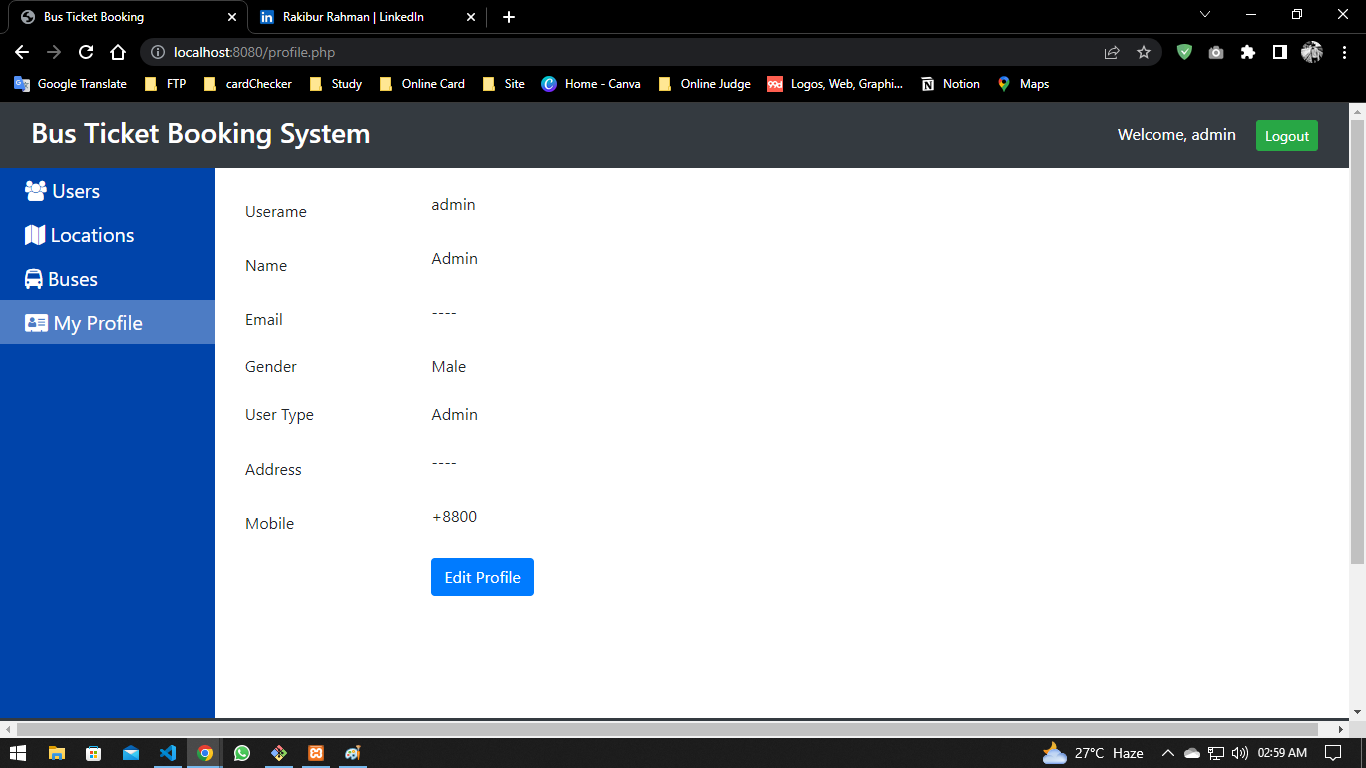
\includegraphics[width=10cm,height=8cm]{img/admin profile view.png}
    \caption{Admin Profile}
    \label{fig:my_label}
\end{figure}
\newpage
\begin{figure}[h]
    \centering
    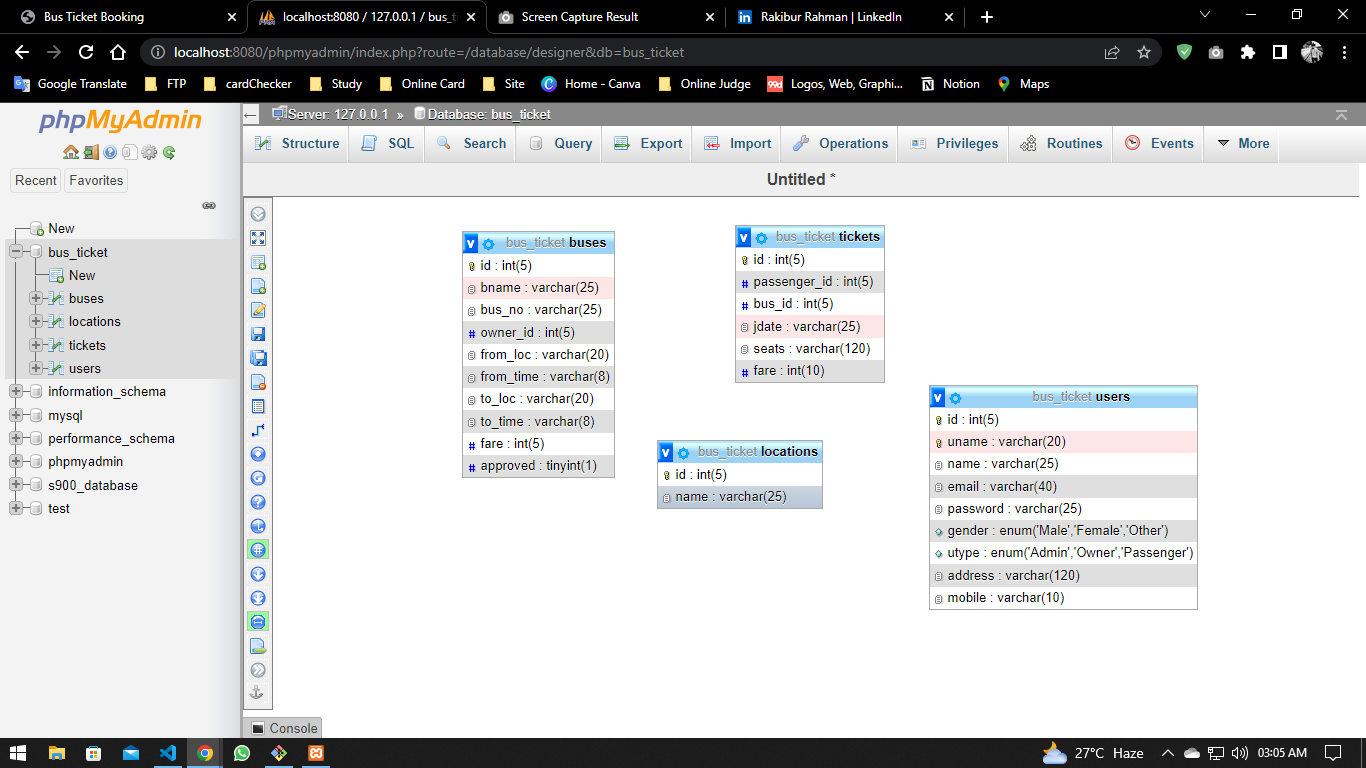
\includegraphics[width=10cm,height=8cm]{img/database.png}
    \caption{Database}
    \label{fig:my_label}
\end{figure}


\chapter*{Conclusion}
Above all it is clear that the modern technology is taking place of everything where possible. It is saving our time and giving us the best benefit of the new era. The above project work is something that can bring up a revolutionary change in online ticket booking systems in my home country Bangladesh. The project is containing in-depth concept and system build up for online air ticket management. \\This system will allow mass users in Bangladesh to book their air ticket online, which is easy, secure and convenient. Whether there are numerous added benefits of this system will helps people in Bangladesh to travel comfortably. Though lacking of software knowledge and information resources might be a problem for this website but future improvement woks. Finally, I honestly hope this project work is just one step for Bangladesh and will bring something new to the online users.
\vspace{1 in}
\begin{thebibliography}{99}
\bibitem{b1} https://www.oreilly.com/library/view/what-is-domain-driven/9781492057802/ch04.html
\bibitem{b2} https://www.shohoz.com/bus-tickets
\bibitem{b3} https://busbd.com.bd/busses
\bibitem{b4} https://www.google.com/forms/about/
\bibitem{b5} https://www.google.com/sheets/about/

\end{thebibliography}

\end{document}